\documentclass[12pt]{article}
\parindent=0.25in

\setlength{\oddsidemargin}{0pt}
\setlength{\textwidth}{440pt}
\setlength{\topmargin}{0in}
\usepackage{amssymb}
\usepackage{amsfonts}
\usepackage{amsmath}
\usepackage{cancel}
\usepackage{latexsym}
\usepackage[center]{subfigure}
\usepackage{epsfig}
\usepackage{3952}
\usepackage{3952-thm}
\usepackage{pstricks,pst-node,pst-tree}
\usepackage{soul, xcolor}
\usepackage{bbold}
\usepackage[backref, colorlinks,citecolor=blue,bookmarks=true]{hyperref}  


% \def\size{\mathop{\rm{size}}\nolimits}
% \def\depth{\mathop{\rm{depth}}\nolimits}
% \newtheorem{theorem}{Theorem}
% \newtheorem{lemma}{Lemma}
% \newtheorem{corollary}{Corollary}
% \newtheorem{fact}{Fact}
% \newtheorem{definition}{Definition}
% \newtheorem{claim}{Claim}
% \newenvironment{proof}{\noindent \textbf{Proof:}}{$\Box$}
% \newenvironment{proofsketch}{\noindent \textbf{Proof Sketch:}}
% \newcommand{\infint}{\int_{-\infty}^\infty}
% \newcommand{\intunit}{\int_{-1}^1}
% \newcommand{\binclass}{x \in \{0,1\}^n}
% \newcommand{\example}{\textbf{Example:} }
% \newcommand{\observation}{\textbf{Observation:} }
% \newcommand{\note}{\textbf{Note:} }
% \newcommand{\noisy}[1]{N_\epsilon(#1)}
% \newcommand{\noisens}[1]{ns_\epsilon(#1)}
% \newcommand{\eg}{{\it e.g.,\ }}
% \newcommand{\Inf}{{\mathrm{Inf}}}
% \newcommand{\PAR}{{\mathrm{PAR}}}
% \def\poly{\mathop{\rm{poly}}\nolimits}
% \def\eps{{\epsilon}}
% \newcommand{\E}{{\bf E}}
% \def\through{{,\ldots,}}


\pagestyle{headings}    % Go for customized headings

\newcommand{\handout}[5]{
   \noindent
   \begin{center}
   \framebox{
      \vbox{
    \parbox[t]{4in} {\bf #1 } \vspace{3mm}  {\hfill \bf #2 }
       \vspace{2mm}
       \hbox to 6.00in { {\Large \hfill #5  \hfill} }
       \vspace{1mm}
       \hbox to 6.00in { {\it #3 \hfill #4} }
      }
   }
   \end{center}
   \vspace*{1mm}
}

\hypersetup{linkcolor=magenta}

\begin{document}

\handout{MATH 3952 (Undergraduate Seminar): Quantum Information Theory}{Spring 2024}
{Organizer: Patrick Lei; Presenter: Tabitha Wan}
{Scribe: Mark Chen}{Lecture 4, Talk 2: February 19, 2024}

\thispagestyle{plain}
% \setcounter{section}{-1}
\section*{Chapter 4 (ctd): Measurements}
\section{Quantum Communication}
\subsection{Basics}
\begin{definition}[Set-Up]
The protocol is for Alice to send quantum states, called \textbf{carriers} to Bob, and Bob needs to identify them by choosing \textbf{appropriate measurements}.
\end{definition}

\begin{remark}
If carriers are described by state vectors in a $2^n$-dimensional Hilbert space, then they can encode at most $n$ bits of information.\\

\noindent Particularly, we start by having Alice and Bob agree upon a basis: $\{\Ket{e_k}\})_{k=1,\ldots, 2^n}$. Then, Alice first chooses one of the $2^n$ states, and Bob can reliable decide distinguish the state chosen for his measurements.
\end{remark}

\begin{remark}\label{rmk:encoding-at-most-log-N-bit-info}
Suppose we are talking about a $2^n$-dimensional Hilbert space defined by the same basis $\{e_k\}_{k=1,\ldots, 2^n}$. It is impossible for Alice to send more than $n$ bits of information by encoding it in $\{\Ket{s_k}\}_{k=1,\ldots, N}$ where $N> 2^n$ and still for Bob to decide his measurements and reliably distinguish between all these states.
\end{remark}

\subsection{Basic Quantum Encoding and Decoding}
Noe, suppose Alice and Bob agreed on the states: $\{\Ket{s_k}\}_{k=1,\ldots, N}$. Alice chooses one of these $N$ states uniformly randomly and send to Bob. Bob tries to perform a measurement defined by the projectors $P_1, \ldots, P_N$.\\

\begin{proposition}\label{prop:projector-on-states}
Suppose $P$ is the projector on the subspace spanned by all signal states, so that $$
P \Ket{s_k} = \Ket{s_k}.
$$ Then, the dimension, \underline{$d$}, of the subspace is $\Trace{P}$
\end{proposition}

\begin{proposition}
Then, the probability that Bob chooses the right $P_k$ to run on $s_k$ is $$
\Pr[\text{success}] = \frac{1}{N}\underset{k}{\sum}\Bra{s_k}P_k\Ket{s_k}.
$$
\end{proposition}
\begin{proof}
This should be very easy to understand. It is just the probability of Alice choosing a specific state $k$ of the $N$ total states times the total probability that Bob guesses correctly.
\end{proof}

\subsubsection{Using Trace Identities}
\begin{proposition}[Recall]\label{prop:prob-to-trace-identity}
$\Bra{s_k} A \Ket{s_k} = \Trace{A\Ket{s_k}\Bra{s_k}}$
\end{proposition}

\begin{proposition}\label{prop:replace-P_k-by-PP_kP}
$\Bra{s_k} P_k \Ket{s_k} = \Bra{s_k}P P_k P\Ket{s_k}$
\end{proposition}
\begin{proof}
Since $P\Ket{s_k} = \Ket{s_k}$, which also means $(\Ket{s_k})^\dag= (P\Ket{s_k})^\dag = \Bra{s_k}P^\dag$. But $P$, as a projector, is a self-adjoint operator, so $P^\dag = P$. This means that $\Bra{s_k} = \Bra{s_k}P$. Therefore, we just replace the appropriate vectors and get $$
\Bra{s_k} P_k \Ket{s_k} = \Bra{s_k}P P_k P\Ket{s_k}
$$
\end{proof}

\begin{theorem}
$\Pr[\text{success}]\leq \frac{d}{N}$
\end{theorem}
\begin{proof}
Notice that, combining proposition \ref{prop:prob-to-trace-identity} and \ref{prop:replace-P_k-by-PP_kP}, we get $$
\begin{aligned}
\Pr[\text{success}]
    &= \frac{1}{N}\underset{k}{\sum}\Bra{s_k} P_k \Ket{s_k}\\
    &= \frac{1}{N}\underset{k}{\sum}\Bra{s_k}P P_k P\Ket{s_k}\\
    &= \frac{1}{N}\underset{k}{\sum}\Trace{P P_k P\Ket{s_k}\Bra{s_k}}\text{, by equality under rotation}
\end{aligned}.
$$

\noindent Notice that $\Trace{BP} \leq \Trace{B}$, because $\exists$ another projector $Q$, by definition, that $$
\begin{aligned}
1
    &= P + Q\\
\implies
\Trace{B}
    &= \Trace{B\cdot 1} = \Trace{B(P+Q)} = \underset{\geq 0}{\underbrace{\Trace{BP}}} + \underset{\geq 0}{\underbrace{\Trace{BQ}}}\\
\implies
\Trace{BP}&\leq \Trace{B}
\end{aligned}.
$$

\noindent Notice that $\kb{s_k}{s_k}$ is all but a projector, so we have: $$
\begin{aligned}
\Pr[\text{success}] = \frac{1}{N}\underset{k}{\sum}\Trace{P P_k P\kb{s_k}{s_k}}
    &\leq \frac{1}{N}\underset{k}{\sum}\Trace{P P_k P}\\
    &= \frac{1}{N}\Trace{P \prt{\underset{k}{\sum}P_k} P}\\
    &= \frac{1}{N}\Trace{P^3}\\
    &= \frac{1}{N}\Trace{P}\text{, $P$ is idempotent}\\
    &= \frac{d}{N}\text{, by end of proposition \ref{prop:projector-on-states}}\\
\implies
\boxed{\Pr[\text{success}]}
    &\boxed{\leq \frac{d}{N}}.
\end{aligned}
$$
\end{proof}

\begin{corollary}\label{cor:encoding-at-most-log-N-bit-info}
This is the reason for remark \ref{rmk:encoding-at-most-log-N-bit-info}. Particularly, if $N> d$, then Bob, even the best he can do, cannot distinguish states with deterministically.
\end{corollary}

\begin{remark}
Another way to say corollary \ref{cor:encoding-at-most-log-N-bit-info} is that, with the current set-up, \hl{one qubit can store at most one bit of information that can reliably be read by a measurement}.\\

\noindent This should be intuitive, because the power of quantum comes from randomness / probability, not deterministic computation.
\end{remark}

\begin{remark}[\textbf{Superdense Codin}g]
There is actually a way for one qubit to store two classical bits, but this relies on Alice and Bob to have a shared entangled start since the beginning of the experiment (to be discussed in chapter 5, section 14, remark 9).
\end{remark}

\subsection{Distinguishing Non-Orthogonal States}
\begin{idea}\label{idea:differentiage-non-orthogonal-signals-how?}
Recall from the second section of talk 1 of this lecture: non-orthogonal states cannot be reliably distinguished. Also, clearly, on the one extreme, we have two states to be orthogonal, then they can be reliably distinguished; on the other extreme, we have two states that are \textbf{collinear}, then Bob cannot distinguish between them at all. So, a key measure of how reliably Bob can distinguish between two states is how close they are to be orthogonal, so, in a sense, it is determined by the angle between the two states:
\begin{center}
    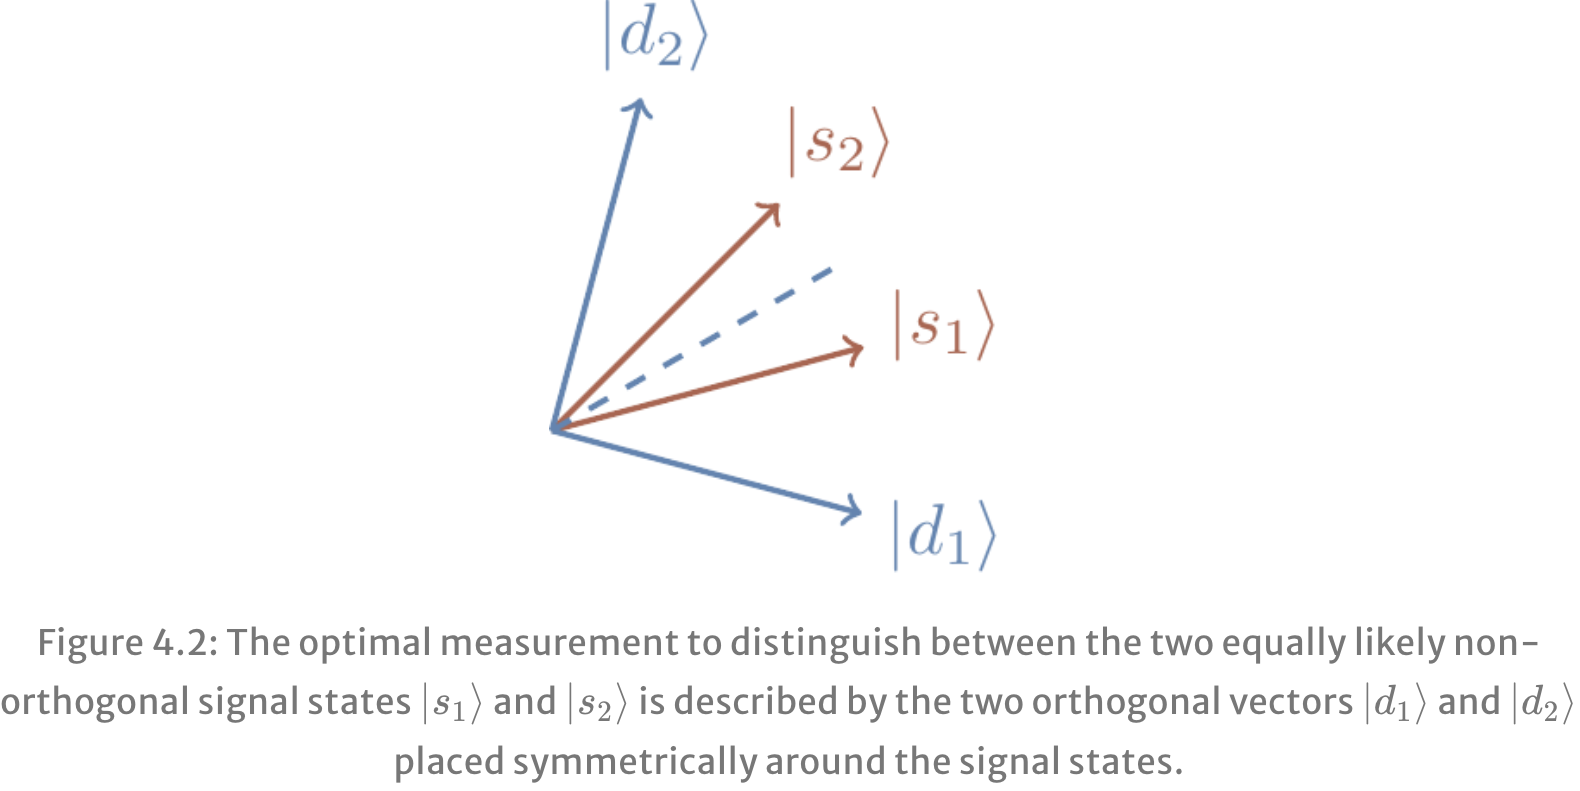
\includegraphics[width = 25em]{images/2.jpg}
\end{center}
\end{idea}

\subsubsection{Suppose a $2$-dimensional Hilbert Space}
\begin{theorem}\label{thm:ubsp2dno}
\hl{(\textbf{Upper Bound of Success Probability to Distinguish Non-Orthogonal Signals}). In this set-up, we have} $$
\boxed{\Pr[\text{success}]\leq \frac{1+\sin(\alpha)}{2}}.
$$
\end{theorem}
\begin{proof}
Say, we have two non-orthogonal, equally likely states, $\Ket{s_1}$ and $\Ket{s_2}$. Bob has two projectors to $P_1, P_2$ that spans the entire subspace spanned by $s_1, s_2$. So, it is the case that $$
P_1 + P_2 = 1.
$$

\noindent As usual, the probability that Bob succeeds is $$
\begin{aligned}
\Pr[\text{success}]
    &= \frac{1}{2}\prt{\Bra{s_1}P_1\Ket{s_1} + \Bra{s_2}P_2\Ket{s_2}}\\
    &= \frac{1}{2}\prt{\Trace{P_1\Ket{s_1}\Bra{s_1}} + \Trace{(1-P_1)\Ket{s_2}\Bra{s_2}}}\\
    &= \frac{1}{2}\prt{\Trace{P_1\Ket{s_1}\Bra{s_1}} + \Trace{\Ket{s_2}\Bra{s_2}} - \Trace{P_1\Ket{s_2}\Bra{s_2}}}\\
    &= \frac{1}{2}\prt{1 + \Trace{P_1\prt{\kb{s_1}{s_1} - \kb{s_2}{s_2}}}}
\end{aligned}
$$

\noindent Next, we study $
D := \kb{s_1}{s_1} - \kb{s_2}{s_2}
$ a little more. We know the following:
\begin{itemize}
    \item It is an operator that acts on the subspace spanned by $s_1, s_2$.
    \item It is Hermitian: $$
    D^\dag = \prt{\kb{s_1}{s_1} - \kb{s_2}{s_2}}^\dag = \kb{s_1}{s_1} - \kb{s_2}{s_2} = D.
    $$
    \item Its eigenvalues add up to $0$: $$
    \underset{k=1,2}{\sum}\lambda_k = \Trace{D} = \Trace{\kb{s_1}{s_1} - \kb{s_2}{s_2}} = \Trace{\bk{s_1}{s_1} - \bk{s_2}{s_2}} = 0.
    $$
\end{itemize}

\noindent Let $\Ket{d_+}$ and $\Ket{d_-}$ be the two orthonormal eigenvectors of $D$, then we let $\pm \lambda$ be their corresponding eigenvalues (again, because we know the eigenvalues add up to $0$), we can rewrite $$
\begin{aligned}
D
    &= \lambda(\kb{d_+}{d_+} - \kb{d_-}{d_-})\\
\implies
\Pr[\text{success}]
    &= \frac{1}{2}\prt{1 + \Trace{P_1 D}}\\
    &= \frac{1}{2}\prt{1 + \lambda\Trace{P_1 (\kb{d_+}{d_+} - \kb{d_-}{d_-})}}
\end{aligned}
$$

\noindent Clearly, since $\lambda\geq 0$, to maximize it we just want to maximize $\Trace{P_1 (\kb{d_+}{d_+} - \kb{d_-}{d_-})}\leq 1$. By simply inspection, we realize that, since $P_1\perp P_2$, we can let:
\begin{itemize}
    \item ($\kb{d_+}{d_+} = P_1$) $$
    \Trace{P_1\kb{d_+}{d_+}} = \Trace{P_1^2} = \Trace{P_1} = 1.
    $$
    \item ($\kb{d_-}{d_-} = P_2$) $$
    \Trace{P_1\kb{d_-}{d_-}} = \Trace{P_1P_2} = \Trace{0} = 0.
    $$
\end{itemize}

\noindent So, \begin{equation}
\Pr[\text{success}] \leq \frac{1}{2}(1+\lambda(1-0)) = \frac{1}{2}(1+\lambda)
\end{equation}
But we already know that the two eigenvalues are $\pm \lambda$, so all we need to do is to find the positive one of the two. That is simple: $$
\begin{aligned}
\Trace{D}
    &= \lambda + (- \lambda)\\
\implies
\Trace{D^2}
    &= (\lambda)^2 + (-\lambda)^2 = 2\lambda^2\\
\text{but also:}
\Trace{D^2}
    &= \Trace{(\kb{s_1}{s_1} - \kb{s_2}{s_2})^2}\\
    &= \Trace{ 2 } - 2\Trace{ \kb{s_1}{s_1}\kb{s_2}{s_2} } = 2- 2\Trace{\bk{s_1}{s_2}\bk{s_2}{s_1}}\\
    &= 2- 2\Trace{|\bk{s_1}{s_2}|^2}\\
\implies
2\lambda^2
    &= 2- 2\Trace{|\bk{s_1}{s_2}|^2}\\
\lambda^2
    &= 1- 1\Trace{|\bk{s_1}{s_2}|^2}\\
\lambda
    &= \pm\sqrt{1 - |\bk{s_1}{s_2}|^2}
\end{aligned}
$$

\noindent But, by definition, we also know that the outcome of $|\bk{s_1}{s_2}|$ is the same as the dot product: $$
|\bk{s_1}{s_2}| = \Ket{s_1}\cdot \Ket{s_2} = |\Ket{s_1}|\cdot |\Ket{s_2}|\cos(\alpha),
$$ where $\alpha$ is the angle between $\Ket{s_1}$ and $\Ket{s_2}$. Notice that $\Ket{s_1}$ $\Ket{s_2}$ both have unit length, so \begin{equation}
|\bk{s_1}{s_2}| = \cos(\alpha) \implies \boxed{\lambda = \pm\sqrt{1-\cos^2(\alpha)} = \pm\sin(\alpha)}
\end{equation}
Since we take $\alpha$ to the smaller angle, $\alpha < \pi\implies \sin(\alpha)\geq 0$, so the positive eigenvalue of the two is \begin{equation}
\lambda = \sin(\alpha).
\end{equation}

\noindent Finally, plug (3) into (1), we get $$
\boxed{\Pr[\text{success}] \leq \frac{1}{2}(1+\lambda) = \frac{1+\sin(\alpha)}{2}}
$$
\end{proof}

\begin{remark}
To make intuitive sense of theorem \ref{thm:ubsp2dno}, just think about the idea \ref{idea:differentiage-non-orthogonal-signals-how?}. It should make a lot of sense at extreme values and in the middle!
\end{remark}

\section{Wiesner's Quantum Money}
The section is not finished on the website.

\section{Quantum Theory, Formally}
\subsection{Axiomatic Quantum Theory}
\begin{idea}
Think about how our quantum computation process has been working: We use vectors to describe quantum states, and matrices (operators) to describe quantum evolutions and measurements. This leads to a convenient mathematical setting for quantum theory: a complex vector space with an inner product (which is exactly a Hilbert space, since we only work in finite dimension).\\

\noindent This is perfectly described by the formalism of the pure math concepts we have used: \underline{Hilbert space, unitary operations, Born's rule, tensor products, etc}. But why?
\end{idea}

\begin{theorem}[Quantum Theory from Five Axioms]
Lucien Hardy's 2008 paper, \href{https://arxiv.org/pdf/quant-ph/0101012.pdf}{Quantum Theory From Five Reasonable Axioms}, shows that, starting from \underline{five axioms}, our choice of formalism is actually the only one that makes sense. And the five axioms are: Let \underline{$K$} be the \textbf{degrees of freedom} (minimum number of real numbers needed to specify a state) and \underline{$N$} be the \textbf{maximum number of states that can be distinguished from each other with one single measurement}.
\begin{itemize}
    \item \textbf{(Probability)} Relative frequency of the outcomes of measuring an ensemble of $n$ systems tend to be well-defined values, when $n\rightarrow \infty$.
    \item \textbf{(Simplicity)} $K$ is a function of $N$, plus minimum number of parameters that would satisfy these axioms.
    \item \textbf{(Subspaces)} For some $M\leq N$, if all states of a system lie within $M$-dimensional subspace, then it should behave exactly like a system of dimension $M$.
    \item \textbf{(Composite systems)} Composite systems behave multiplicative, i.e. if a system is a composite of two subsystems $A$ and $B$, then $N = N_A N_B$ and $K = K_AK_B$.
    \item \textbf{(Continuity)} Given any two \textbf{pure states} (all of the states that we have been discussing so far are pure states, but we define what this means in section 8.1) of a system, $\exists$ a continuous reversible transformation of the system that sends one to the other.
\end{itemize}
\end{theorem}

\begin{remark}
For example, if we drop ``continuous" from the fifth axiom, then it is exactly the same as classical probability.
\end{remark}

\subsection{Quantum States from Hilbert Space (Revisited)}
\begin{proposition}
Any isolated quantum system with $n$ perfectly distinguishable states can be associated with a Hilbert space $\HHH$ of dimension $n$ such that each $\Ket{v}\in HHH$ of unit length $\bk{v}{v} = 1$ represents a quantum state of the system.
\end{proposition}

\begin{proposition}[Recall Some Properties] $\bk{u}{v}$ gives the probability amplitude of starting in state $\Ket{v}$ and end in $\Ket{u}$. If $\bk{u}{v} = 0\implies$ $\Ket{u}$ and $\Ket{v}$ are perfectly distinguishable. States that form orthonormal bases are always perfectly distinguishable from each other.
\end{proposition}

\subsection{Quantum Evolutions (Revisited)}
Any physically admissible evolution of an isolated quantum system is represented by a \textbf{unitary operator}. These unitary operators are usually derived from \textbf{Schrödinger's Equation}: $$
\frac{d}{dt}\Ket{\psi(t)} = -\frac{i}{\hbar}\hat{H}\Ket{\psi(t)},
$$ where \underline{$\hat{H}$} is a \textbf{Hermitian operator} called the \textbf{Hamiltonian}.

\begin{proposition}
The \textbf{Schrödinger's Equation} contains a complete specification of all interactions both \underline{within the system} and \underline{between the system and the external potentials}.
\begin{itemize}
    \item (For time-dependent Hamiltonians) The formal solution of the Schrödinger's Equation is $$
    \Ket{\psi(t)} = U(t)\Ket{\psi(0)}, U(t) = e^{-\frac{i}{\hbar}\hat{H}t}.
    $$
    \item Any unitary matrix can be written as the exponential of \underline{some Hermitian matrix $\hat{H}$} and \underline{some real coefficient $t$}: $$
    \boxed{e^{it\hat{H}} = 1-it\hat{H} + \frac{(-it)^2}{2}\hat{H}^2 + \frac{(-it)^3}{2\cdot 3}\hat{H}^3 + \cdots = \Sum{n}{0}{1}\frac{(-it)^n}{n!}\hat{H}^n}.
    $$ [For example, for very small $t$, this should be arbitrarily close to the unit operator $1$.]
\end{itemize}
\end{proposition}

\subsection{Quantum Circuits with Quantum Gates}
To implement and use certain unitary operations to construct other more complex unitaries.

\subsection{Measurements}
A complete measurement in quantum theory is determined by the choice of an orthonormal basis $\{\Ket{e_{k}}\}_{k= 1,\ldots, n}\subseteq \HHH$, and every such basis represents a possible measurement (in principle).

\begin{proposition}\label{prop:decomp-identity-probability-unitary}
For any decomposition of the identity into projectors $$
1 = \underset{k}{\sum} P_k,
$$ $\exists$ a measurement that takes a quantum system in state $\Ket{\psi}$, outputs label $k$ with probability $\Bra{\psi}P_k\Ket{\psi}$, and leaves the system in state $P_k\Ket{\psi}$. This is described by $$
\Ket{\psi}\mapsto \frac{P_k\Ket{\psi}}{\sqrt{\Bra{\psi}P_k\Ket{\psi}}}
$$
\end{proposition}

\begin{remark}
The projector formalism as described in proposition \ref{prop:decomp-identity-probability-unitary} covers both complete and incomplete measurements. Complete measurements are exactly the ones defined by rank-one projectors $$
P_k = \kb{e_k}{e_k},
$$ \hl{i.e. projecting on vectors from some orthonormal basis $\{\Ket{e_k}\}_{k=1, \ldots, n}$}.
\end{remark}

\end{document}